\section{Results}\label{sec:qanalysis}

This section shows the analysis and discussion of our Systematic Mapping results.
We proceed by presenting bubble charts as result of combining different facets in order to 
\textit{(i)} answer the research questions and \textit{(ii)} to justify our proposal.


\subsection{Quantitative Analysis}


Our analysis presents the frequencies of publications for
the choosen facets. The results are presented in bubble charts. The
charts show the aggregated view of the number of papers  considering the facets. 
% Despite the low number of works tackling other publishers, they maintain their
% presence over the years, mainly between 2008-2014. IEEE and ACM are the publishers
% that most published papers related to service-oriented applications considering
% non-functional properties. Considering Elsevier, we can found papers only from 2008.
% Figure 1a presents the publications for each publisher per year.


\subsubsection{Combining the facets Contribution, SLA and Data Integration
Description:}

\begin{figure}[h!]
\centering
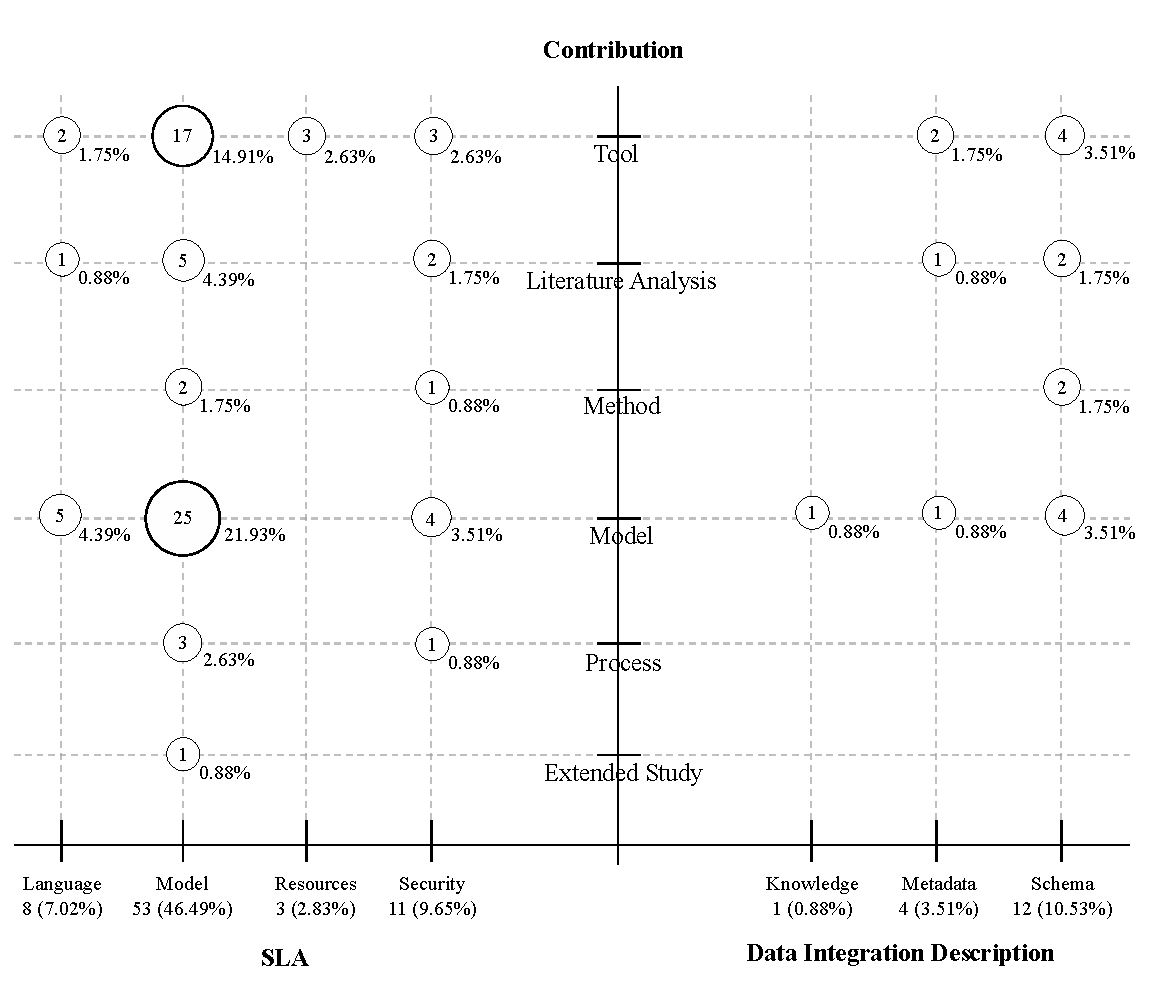
\includegraphics[scale=0.56]{figs/bubble-charts/Contribution-SLA-DIdescription.pdf} 
\caption{Contribution, SLA and Data Integration Description}\label{fig:facet1}
\end{figure}

Combining the facet contribution with the facets SLA and data integration description 
(Figure~\ref{fig:facet1}) it is possible to obtain two analysis: 
(i) how the SLA has been applied to scientific works and which are the type of contribution 
most proposed by the authors; and (ii) which are the most applied data integration description
strategy in papers and which are the most type of contribution associated to these works. 
Looking to the figure you can note that models for SLA have been the focus in the papers 
(53 appearances - 46.49\%) followed by Security (11 appearances - 9.65\%), Language 
(8 appearances - 7.02\%) and Resources (3 appearances - 22.83\%).
Analyzing the figure is also possible to observe that Model (34 appearances - 29.82\%) and 
Tool (25 appearances - 21.93\%) are the mainly type of contribution proposed in the papers 
followed by Literature Analysis (8 appearances - 7.02\%), Process (4 appearances - 3.51\%), 
Method (3 appearances - 2.63\%) and Extended Study (1 appearance - 0.88\%).
Regarding the data integration description, Schema (12 appearances - 10.53\%) is the most 
applied dimension followed by Metadata (4 appearances - 3.51\%) and Knowledge (1 appearance - 0.88\%).

\subsubsection{Combining the facets Data Integration Environment, Contribution
and Research:}

\begin{figure}[h]
\centering
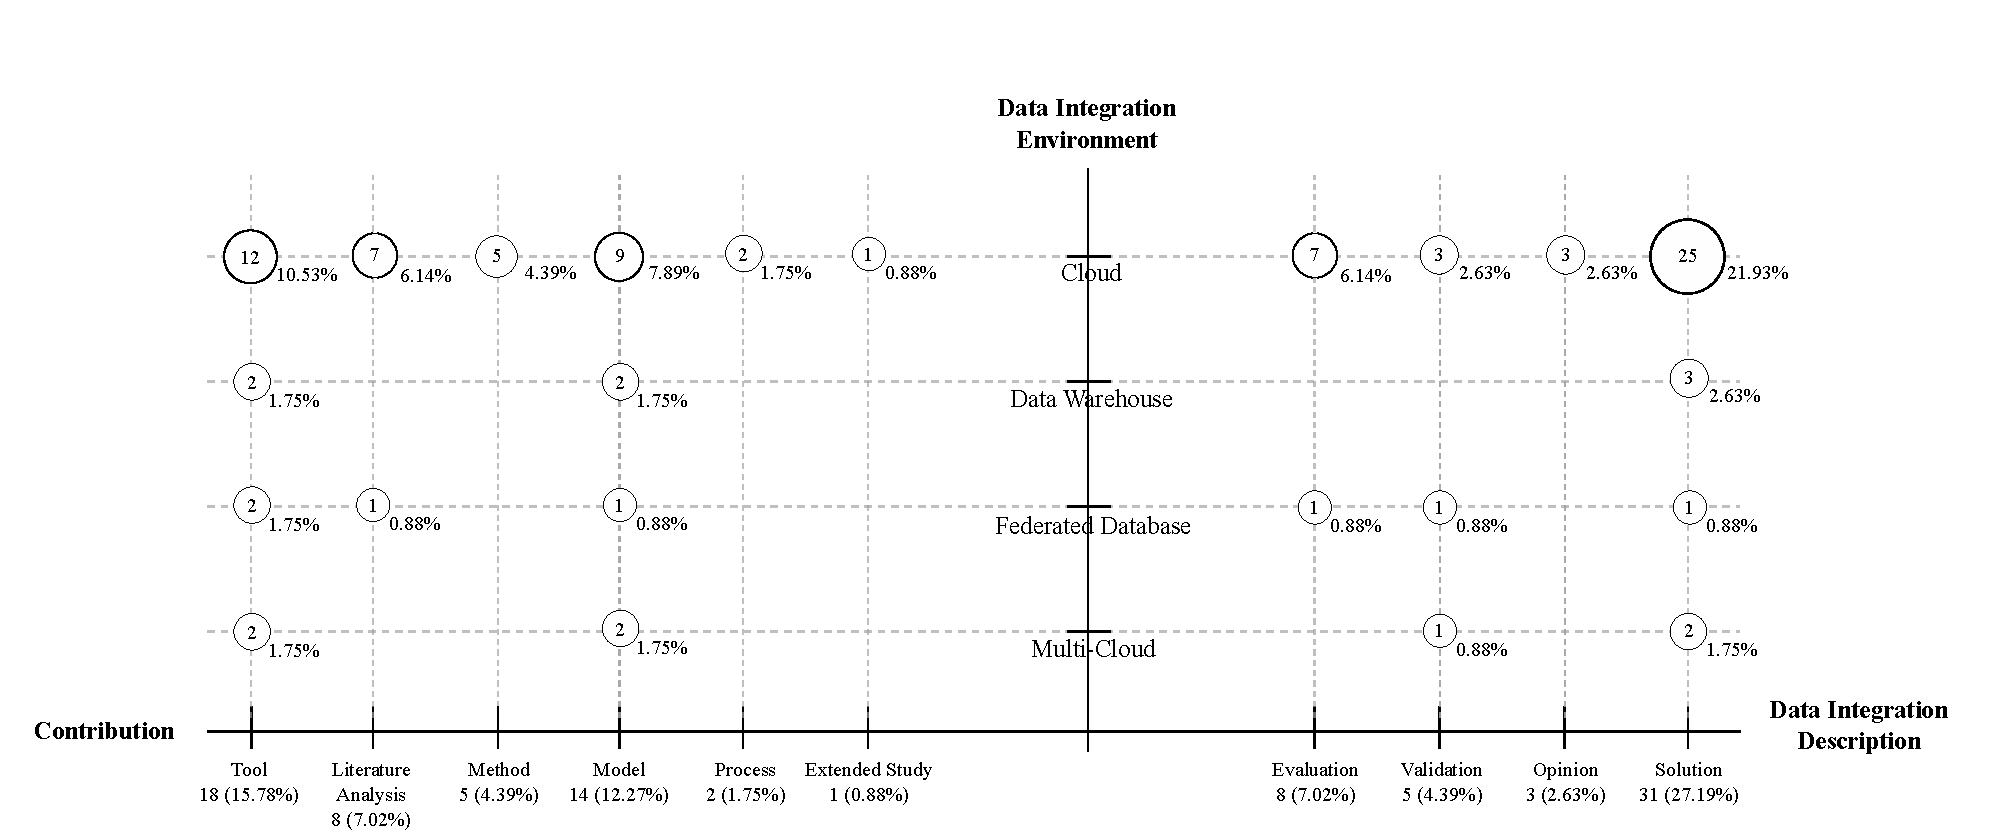
\includegraphics[scale=0.48]{figs/bubble-charts/DI-Environment-Contribution-Research.pdf}
\caption{facets Data Integration Environment, Contribution and Research}\label{fig:facet2}
\end{figure}

Combining the facet data integration environment with the facets contribution and research 
(Figure~\ref{fig:facet2}) it is possible to observe which are the most proposed type of
contribution and research applied to the different data integration environments.  
Looking to the figure it is possible to identify that Tool (18 appearances - 15.78\%) and 
Model (14 appearance - 12.27\%) are the mainly type of contribution developed, 
followed by Literature Analysis (8 appearances - 7.02\%), Method (5 appearances - 4.39\%) 
Process (2 appearances - 1.75\%) and Extended Study (1 appearance - 0.88\%).
Analyzing the figure is also possible to observe that Solution (31 appearances - 27.19\%) is 
the type of research most proposed, followed by Evaluation (8 appearances -
7.02\%), Validation (5 appearances - 4.39\%) and Opinion (3 appearances - 2.63\%).

\iplacido{`Old' figure 3 deleted\ldots} 
 
% \subsection{Combining the facets SLA and Contribution}
% 
% Combining the facet SLA with the facet contribution (Figure~\ref{fig:facet3}) it is possible 
% to observe how the SLA has been applied to scientific works and which are the type of contribution 
% most proposed by the authors.
% Looking to the figure you can remark that models for SLA have been the focus of the most papers 
% (53 appearances).
% Analyzing the figure is also possible to observe that Model (34 appearances - 29.82\%) and 
% Tool (25 appearances - 21.93\%) are the mainly type of contribution proposed in the papers 
% followed by Literature Analysis (8 appearances - 7.02\%), Process (4 appearances - 3.51\%), 
% Method (3 appearances - 2.63\%) and Extended Study (1 appearance - 0.88\%).
% 
% \begin{figure}[h!]
% \centering
% 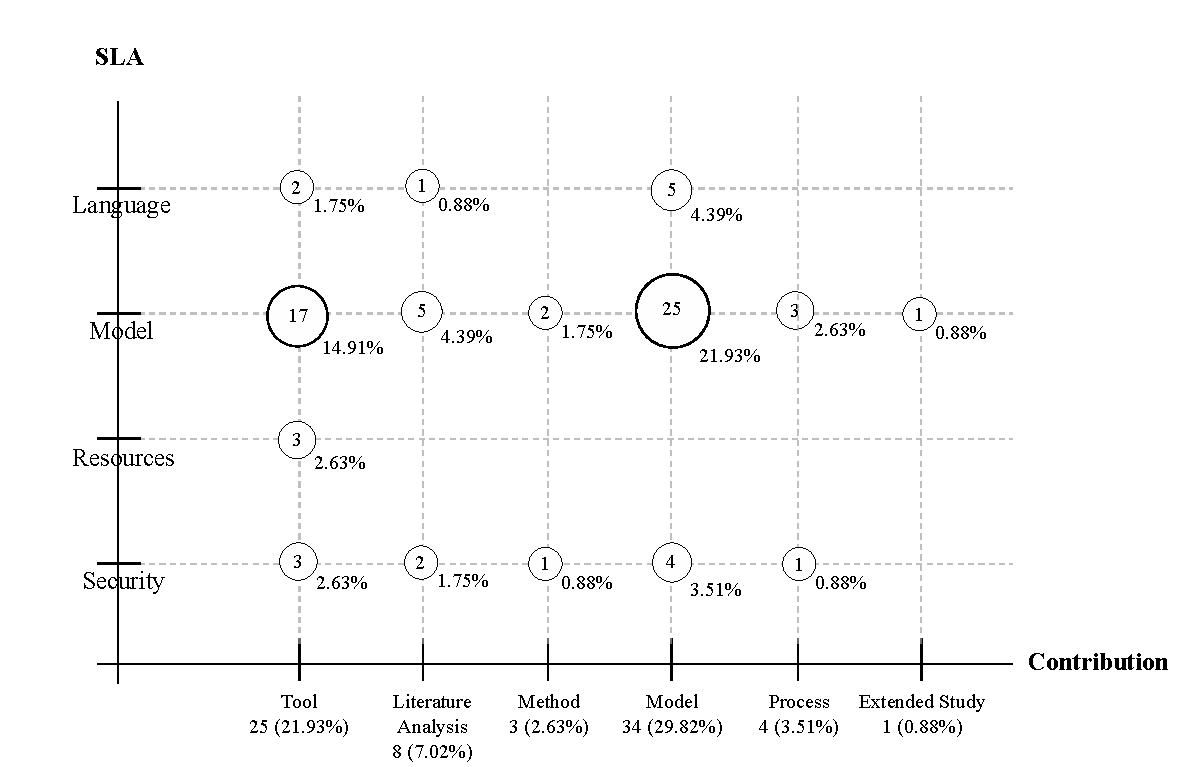
\includegraphics[scale=0.65]{figs/bubble-charts/SLA-Contribution.pdf}
% \caption{Facets SLA and Contribution}\label{fig:facet3}
% \end{figure}


\subsubsection{Combining the facets Data Quality, Data Integration Environment
and Data Integration Description:}

Combining the facet data quality with the facets data integration environment and data integration description
(Figure~\ref{fig:facet4}) it is possible to note which quality of service parameters have been applied most in
data integration studies.
It is also possible to identify which are the most applied data integration environment and description.
First of all, security and privacy are the most applied QoS parameter (5 appearance - 4.39\%)
followed by the other dimensions (1 appearance - 0.88\%). 
The figure also shows that SLA has not been widely used in order to address data integration solutions
(1 appearance) which reinforces our main objective of integrate SLA, data integration and multi-cloud 
environments. 
Analyzing the figure is also possible to observe that the most deployed data integration environment is 
the cloud (9.68\%) followed by multi-cloud (4.39\%), federated databases (1.75\%) and data warehouse (0.00\%).
The data integration description dimensions had the same percentage for schema, knowledge and metadata (2 appearance - 1.75\%)

\begin{figure}[!h]
\centering
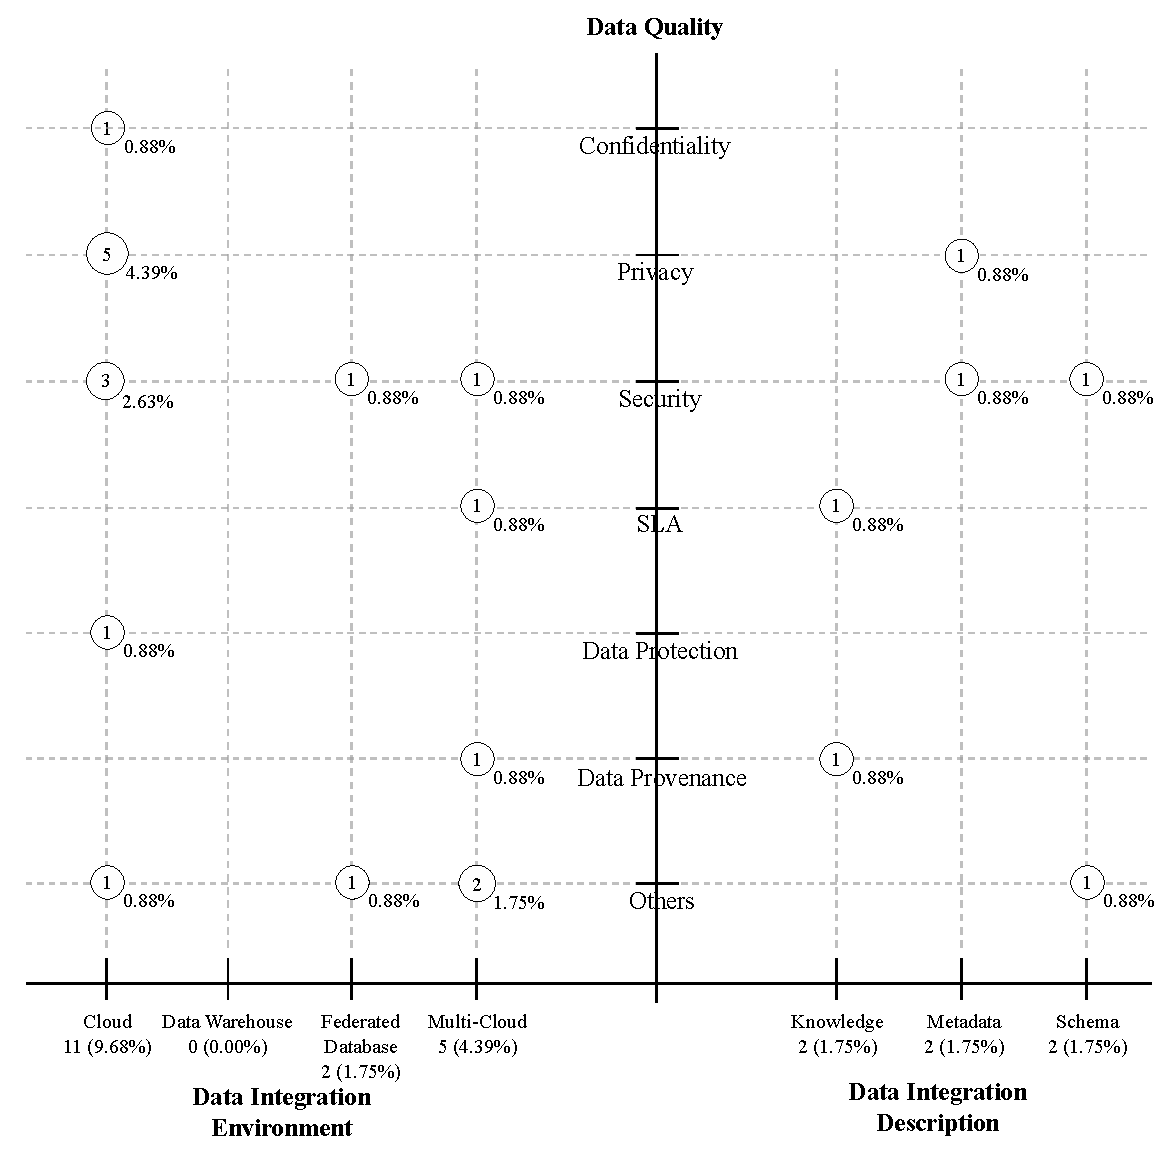
\includegraphics[scale=0.53]{figs/bubble-charts/Data-Quality-DI.pdf}
\caption{Facets Data Quality, Data Integration Environment and Data Integration Description}\label{fig:facet4}
\end{figure}

\subsection{RQ1: Which are the SLA measures that have been applied most in
the cloud?}

\subsection{RQ2: How has the publication of papers on data integration
involved towards cloud topics?}


\subsection{RQ3: How and in which context have data integration guided by QoS
models or requirements been explored in the literature?}